%\documentclass[10pt,twocolumn,letterpaper,draft]{article}
\documentclass[10pt,letterpaper]{ctexart}

\usepackage{cvpr}
% \usepackage{epsfig}
\usepackage{graphicx}
\usepackage{amsmath}
\usepackage{amssymb}
% \usepackage{color}
\usepackage{subfigure}
\usepackage{algorithm}
\usepackage{algorithmicx}
\usepackage{algpseudocode}
\usepackage{pythonhighlight}
\usepackage{xcolor}
\usepackage{listings}
\lstset{language=C++,
    basicstyle=\ttfamily,
    frame=single,
    keywordstyle=\color{blue}\ttfamily,
    stringstyle=\color{magenta}\ttfamily,
    commentstyle=\color{green}\ttfamily,
    morecomment=[l][\color{magenta}]{\#},
    morekeywords={*,__int64}
}

\renewcommand{\labelenumi}{\alph{enumi}.} % Make numbering in the enumerate environment by letter rather than number (e.g. section 6)
\floatname{algorithm}{算法}
\renewcommand{\algorithmicrequire}{\textbf{输入:}}
\renewcommand{\algorithmicensure}{\textbf{输出:}}

\usepackage{enumitem}
\setenumerate[1]{itemsep=0pt,partopsep=0pt,parsep=\parskip,topsep=5pt}
\setitemize[1]{itemsep=0pt,partopsep=0pt,parsep=\parskip,topsep=5pt}
\setdescription{itemsep=0pt,partopsep=0pt,parsep=\parskip,topsep=5pt}

% Include other packages here, before hyperref.

% If you comment hyperref and then uncomment it, you should delete
% egpaper.aux before re-running latex.  (Or just hit 'q' on the first latex
% run, let it finish, and you should be clear).
\usepackage[pagebackref=true,breaklinks=true,letterpaper=true,colorlinks,bookmarks=false]{hyperref}


\cvprfinalcopy % *** Uncomment this line for the final submission

\def\cvprPaperID{159} % *** Enter the CVPR Paper ID here
\def\httilde{\mbox{\tt\raisebox{-.5ex}{\symbol{126}}}}

\newcommand{\mypara}[1]{\paragraph{#1.}}

\graphicspath{{figures/}}

% Pages are numbered in submission mode, and unnumbered in camera-ready
%\ifcvprfinal\pagestyle{empty}\fi
\setcounter{page}{1}


%\begin{CJK*}{GBK}{song}

\newcommand{\figref}[1]{图\ref{#1}}
\newcommand{\tabref}[1]{表\ref{#1}}
\newcommand{\equref}[1]{式\ref{#1}}
\newcommand{\secref}[1]{第\ref{#1}节}

\ctexset{
  section={
          name={,、},
          number={\chinese{section}},
          format={\heiti},
          beforeskip={0.1ex},
          afterskip={0.1ex},
          aftername={\nobreak},
          indent={\parindent},
          },
}
\usepackage{zhnumber}

\newcommand\zhsubsec[1]{{% 中文小节
\bfseries{
\stepcounter{subsection}(\zhnum{subsection}){#1}}
\vspace{0.1pt}%
}}

%%%%%%%%% TITLE

% \begin{algorithm}
%   \caption{题注}
%     \begin{algorithmic}[1] %每行显示行号
%         \Function {$Function name$}{$parameters$}
%
%         \EndFunction
%     \end{algorithmic}
% \end{algorithm}

\begin{document}
\pagestyle{plain}
\title{
    \begin{center}
        \phantom{Start!}
    	  \vspace{2cm}
        \center{\zihao{1} 中山大学数据科学与计算机学院}
        \center{\zihao{2} 计算机科学与技术专业-人工智能}
        \center{\zihao{2} 本科生实验报告}
        \center{(2018-2019学年秋季学期)}
    \end{center}
}
\maketitle

\begin{center}
    \setlength{\baselineskip}{40pt}
    \vspace{1cm}
    \zihao{-2}
    \center{
        \begin{tabular}{cc}
      	学\qquad 号:& \underline{~~~~~~16337113~~~~~~}  \\
      	姓\qquad 名:& \underline{~~~~~~~劳马东~~~~~~~}  \\
        教学班级:   & \underline{~~~~~教务2班~~~~~}  \\
      	专\qquad 业:& \underline{~~~~~~~~~超算~~~~~~~~}  \\
      	\end{tabular}
    }
\end{center}
\pagebreak

%%%%%%%%% BODY TEXT %%%%%%%%%%%%%%%%%%%%%%%%%%%%%%%%%%%%%%%%
\section{实验题目}
\begin{enumerate}[itemindent=1.5em,label=\arabic*、]
  \item 使用A*与IDA*算法解决15-Puzzle问题,启发式函数可以自己选取,最好多尝试不同的启发式函数;
  \item 代码要求使用python或者C++;
  \item 报告要求
  \begin{enumerate}
    \item 报告中需要包含对两个算法的原理解释
    \item 需要包含性能和结果的对比和分析
    \item 如果使用了多种启发式函数,最好进行对比和分析
    \item 需要在报告中分情况分析估价值和真实值的差距会造成算法性能差距的原因
  \end{enumerate}
\end{enumerate}

\section{实验内容}
\zhsubsec{算法原理}
\begin{enumerate}[itemindent=2.5em,label=\arabic*、]
    \item 拼图问题的形式化
    \begin{enumerate}[itemindent=1.5em,label=(\arabic*)]
        \item 问题定义
        \begin{itemize}
            \item 初始状态
            \item 行动
            \item 状态空间
            \item 目标测试
            \item 路径耗散
        \end{itemize}
        \item 问题的解:序列
    \end{enumerate}
\end{enumerate}
\zhsubsec {关键代码}

\begin{lstlisting}
// 用于表示数码的位数,0-15一个数字只需4位
#define BITWISE 4
// 1111,用于取低4位
#define LOWERBIT 15
class Puzzle {
  // 16个数刚好用去64位
  __int64 _puzzle;
public:
  const int dim_size;

  Puzzle(int numbers) : dim_size(sqrt(numbers + 1) + 0.5), _puzzle(0) { }

  // 实现类似于二维数组下标索引的get、set接口
  int get(int i, int j) const {
      // 计算偏移量,与位数相乘,得到(i,j)元素最低位的地址
      i = (i * dim_size + j) * BITWISE;
      // 右移,取低4位就是(i,j)元素
      return (_puzzle >> i) & LOWERBIT;
  }

  void set(int i, int j, int x) {
      __int64 x64 = LOWERBIT;;
      int offset = (i * dim_size + j) * BITWISE;
      // 先将(i,j)元素置为0
      _puzzle &= ~(x64 << offset);
      x64 = x;
      // 左移取或就能把(i,j)置为x
      _puzzle |= (x64 << offset);
  }
}
\end{lstlisting}
  % \begin{figure}[H]
  % \centering
  % \subfigure[DLS]{
  % 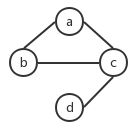
\includegraphics[width=0.3\textwidth]{dls-0.PNG}
  % \label{fig:dls}}
  % \subfigure[IDS]{
  % 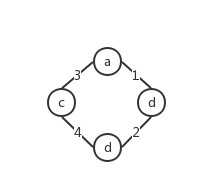
\includegraphics[width=0.3\textwidth]{dfs-2.PNG}
  % \label{fig:ids}}
  % \end{figure}

\newpage
\section{实验结果及分析}
\zhsubsec{实验结果展示}

\zhsubsec{评测指标展示及分析}
\begin{table}
  \centering
  \caption{运行时间(/秒)}
  \label{table:time}
  \begin{tabular}{c|c|c|c|c}
  \hline
  搜索策略 & 样例1 & 样例2 & 样例3 & 样例4\\
  \hline
  A* & 550 & 14 & 808 & 39 \\
  \hline
  \end{tabular}
\end{table}

\begin{table}
  \centering
  \caption{生成节点数}
  \label{table:time}
  \begin{tabular}{c|c|c|c|c}
  \hline
  搜索策略 & 样例1 & 样例2 & 样例3 & 样例4\\
  \hline
  A* & 81004390 & 2662191 & 117201754 & 6927246 \\
  \hline
  \end{tabular}
\end{table}
\section{思考题}

\end{document}
